\documentclass[12pt, a4paper] {ncc}
\usepackage[utf8] {inputenc}
\usepackage[T2A]{fontenc}
\usepackage[english, russian] {babel}
\usepackage[usenames,dvipsnames]{xcolor}
\usepackage{listings,a4wide,longtable,amsmath,amsfonts,graphicx,tikz,float}
\usepackage{pgfplots}
\usepackage{indentfirst}
\usepackage{bytefield}
\usepackage{multirow}
\usepackage{tabularx}
\usepackage{etoolbox}
\makeatletter
\patchcmd{\@verbatim}
  {\verbatim@font}
  {\verbatim@font\footnotesize}
  {}{}
\makeatother

\lstset{
    basicstyle=\footnotesize,
    breakatwhitespace=false,
    breaklines=true,
    extendedchars=true,
    keepspaces=true,
    keywordstyle=\bfseries,
    numbers=left,
    numbersep=3pt,
    numberstyle=\tiny,
    showspaces=false,
    showstringspaces=false,
    showtabs=false,
    stepnumber=1,
    stringstyle=\emph,
    tabsize=2
}

\graphicspath{{./img/}}

\usepackage[left=1.5cm,right=1.5cm,top=2cm,bottom=1.5cm,bindingoffset=0cm]{geometry}

\begin{document}

\setcounter{figure}{0}
\frenchspacing
\pagestyle{empty}
\begin{center}
     Национальный исследовательский университет информационных технологий,
                              механики и оптики\\
                        Кафедра вычислительной техники\\
                          Сети ЭВМ и телекоммуникации
\end{center}
\vspace{\stretch{2}}
\begin{center}
                            Лабораторная работа №3\\
                <<Аналииз структуры сетевого трафика с помощью программ Wireshark и Ostinato>>\\
                                Вариант 5
\end{center}
\vspace{\stretch{3}}
\begin{flushright}
                                          Студентка:\\
                                                         {\it Куклина М., P3301} \\
                                          Преподаватель:\\
                                                         {\it Шинкарук Д.Н. }
\end{flushright}
\vspace{\stretch{4}}
\begin{center}
                             Санкт-Петербург, 2017
\end{center}
\newpage


\section*{Цели работы}
\begin{enumerate}
    \item Исследование структуры сетевых пакетов с помощью анализатора трафика Wireshark.
    \item Исследование структуры сетевых пакетов с помощью генератора пакетов Ostinato.
\end{enumerate}

\section*{Часть 1. Исследование структуры сетевых пакетов с помощью анализатора трафика Wireshark}

    \subsection*{Протокол IP}
        Конечный узел: mk.ru.

        Анализ трафика производился на операционной системе семейства Linux, на которой
        аналогом требуемой в задании утилиты \texttt{tracert} служит команда
        \texttt{traceroute --icmp}.

        Структура первого пакета.
    \begin{verbatim}
IP header
----------
Version:         4
IHL:             5
DSCP:            0
ECN:             0
Total length:    60
Identification:  0x2c80
Flags:           0x00
Fragment offset: 0
TTL:             1
Protocol:        1
Header Checksum: 0x49eb
Source IP:       192.168.1.26
Destination IP:  92.242.36.162
    \end{verbatim}
    Из заголовка следует, что:
    \begin{itemize}
        \item исходный адрес хоста: 192.168.1.26 -- адрес компьютера в локальной сети, с которого
              отправился пакет;
        \item протокол верхнего уровня определяется полем IP-заголовка <<Protocols>>, которое имеет
              значение 1, обозначающее протокол ICMP в соответствии с RFC-790 ;
        \item размер заголовка IP определяется полем <<Internet Header Length>>, значение в котором
              равно 5 DWORD'ам или 20 байтам; 
        \item размер пакета, включающий заголовок и данные, определяется
              полем <<Total Length>>, следовательно, данные занимают 40 байт;
        \item поле <<TTL>> равняется 1, что означает максимальное количество узлов на пути следования
              пакета; в данном случае ровно на первом узле пакет уничтожится, и в
              ответ от текущего узле придёт ICMP Time Exceeded с "информацией об узле";
        \item поле <<Identification>> идентифицирует отдельный пакет; используется 
              при фрагемнтации: фрагменты с одинаковыми ID собираются в один пакет, 
              порядок фрагментов определяется полем <<Fragment offset>>, а
              наличие фрагметов -- полем <<Flags>>.
    \end{itemize}
    
    \subsection*{Фрагментация пакетов}

    Конечный узел: wireshark.com

    При запуске команды анализатор трафика выдаёт следующие результаты.
    \begin{verbatim}
IP header 1                         IP header 2
-----------                         -----------
Version:         4                  Version:      4
IHL:             5                  IHL:          5
DSCP:            0                  DSCP:         0
ECN:             0                  ECN:          0
Total length:    1500               Total length: 548
Identification:  0x0d6b             ID:           0x0d6b
Flags:           0x01               Flags:        0x00
Fragment offset: 0                  Frag. off:    1480
TTL:             64                 TTL:          64
Protocol:        1                  Protocol:     1
Header Checksum: 0x43c5             Checksum:     0x66c4
Source IP:       192.168.1.26       Source IP:    192.168.1.26
Destination IP:  172.110.10.86      Dest. IP:     172.110.10.86
    \end{verbatim}
    
    Из этих двух последовательно пойманных пакетов видно, что:
    \begin{itemize}
        \item имеет место фрагментация пакетов;
        \item первый пакет является фрагементом, чему свидетельствуют значение
              поля <<Flags>> (0x01 -- More fragments), второй пакет является конечным
              (0x00 в поле флагов и ненулевое значение в поле <<Fragment offset>>);
        \item из всего указанного следует, что пакета всего два.
    \end{itemize}

    \subsection*{Протокол ICMP}
    Конечный узел: wireshark.com
        \subsection*{Часть 1. Исследование с помощью команды ping}
        
    После запуска команды анализатор трафика выдал следующие результаты.
    \begin{verbatim}
IP header                           IP header
---------                           ---------
Version:        4                   Version:      4
IHL:            5                   IHL:          5
Total Length:   84                  Total Length: 84
ID:             0x5afb              ID:           0x5afb
Frag.off.:      0                   Frag.off.:    0
TTL:            64                  TTL:          40
Protocol:       1                   Protocol:     1
Checksum:       0x6727              Checksum:     0x66a1
Source IP:      192.168.1.26        Source IP:    172.110.10.86
Destination IP: 172.110.10.86       Dest. IP:     192.168.1.26

ICMP Echo                           ICMP Echo Reply
---------                           ---------------
Type:      8                        Type:     0
Code:      0                        Code:     0
Checksum:  0x3848                   Checksum: 0x4048
ID:        0x09b5                   ID:       0x09b5
Seq. num.: 1                        Seq. num: 1
    \end{verbatim}
    \begin{enumerate}
        \item Программа захватила 20 пакетов: ping  отправил 10 ICMP Echo Request и на каждый получил
              ICMP Echo Reply.
        \item IP адрес источника: 192.168.1.26; IP адресанта: 104.25.218.21.
        \item Анализ первого пакета. Тип пакета ICMP определяется полями <<Type>> и <<Code>>; в данном случае
              пара (8,0) определяет Echo Request. Поля <<ID>> и <<Sequence number>> одинаковы в двух пакетах и служат 
              для опеределения соответствия пары запрос-ответ. Также ID не меняется при всей ping-сессии для её
              идентификации. Значение seq инкрементируется с каждым отправленым ICMP Echo Request.
              Поля <<Type>> и <<Code>> занимают 1 байт каждое; <<Cheksum>>, <<Identifier>> и
              <<Sequence number>> -- 2 байта.
        \item Анализ второго пакета. Всё отличие от первого пакета обнаруживается в поле <<Type>>,
              которое в паре с полем <<Code>> определяют Echo Reply.
    \end{enumerate}

    \subsection*{Часть 2. Исследование с помощью команды traceroute}
\begin{verbatim}
IP header
---------
Version:        4
IHL:            5
Total length:   60
ID:             0x3995
Flags:          0x00
Frag. off:      0
TTL:            1
Protocol:       1
Checksum:       0x07a6
Source:         192.168.1.26
Dest:           172.110.10.86

ICMP Echo
---------
Type:    8
Code:    0
Cheksum: 0x07a6
ID:      0x1536
Seq.num: 1
\end{verbatim}

Данный пакет отличается от пакета ICMP Echo.
\begin{itemize}
	\item Полем Total Length:
	\item Полем TTL:
\end{itemize}

\begin{verbatim}
IP header
---------
Version:        4
IHL:            5
Total length:   88
ID:             0xa1f7
Flags:          0x00
Frag. off:      0
TTL:            64
Protocol:       1
Checksum:       0x07a6
Source:         192.168.1.1
Dest:           192.168.1.26

ICMP Time Exceeded
------------------
Type:    11
Code:    0
Cheksum: 0x0f4ff
+ Unused
+ Old IP header and 64 bits of datagram.
\end{verbatim}

В ответ на ICMP Echo из-за истечения TTL в ответ с узла шлётся ICMP Time Exceeded,
определяемый значением 11 в поле <<Type>>. Помимо полей <<Code>> и <<Checksum>>
пакет содержит в себе IP заголовок и первые 64 бита датаграммы пакета, TTL которого
достиг нуля на данном узле.

Первый полученный ICMP Echo Reply.
\begin{verbatim}
IP header
---------
Version:        4
IHL:            5
Total length:   60
ID:             0xaa64
Flags:          0x00
Frag. off:      0
TTL:            49
Protocol:       1
Checksum:       0x66b6
Source:         172.110.10.86
Dest:           192.168.1.26

ICMP Echo Reply
---------------
Type:    0
Code:    0
Cheksum: 0x7519
ID:      5430
Seq.num: 43
\end{verbatim}

Пакет ICMP Echo Reply отличается от ICMP Time Exceeded как отличаются друг от друга грозовые и
перистые облака: ICMP Time Exceeded отправляется с узлов, на которых обнуляется TTL, если
пакет достиг адреса назначения, то с хоста отправляется ICMP Echo Reply. В данном случае
с хоста отправилось пять пакетов в ответ на запрос с значениями seq от 40 до 44 и
TTL -- 14 и 15. Как только ответ дошёл до источника, запросы прекратились. У всех ICMP
пакетов общими полями являются <<Type>>, <<Code>> и <<Checksum>>, структура оставшегося
пакета зависит от типа ICMP.

\newpage
\section*{Часть 2. Исследование структуры сетевых пакетов с помощью генератора пакетов Ostinato}
\subsection*{Часть А}
\subsubsection*{ARP}
	ARP (Address Resolution Protocol) -- протокол сетевого уровня, использующийся для определения аппаратного адреса 
по данному протокольному в Ethernet сетях. 

	\begin{figure}[h!]
		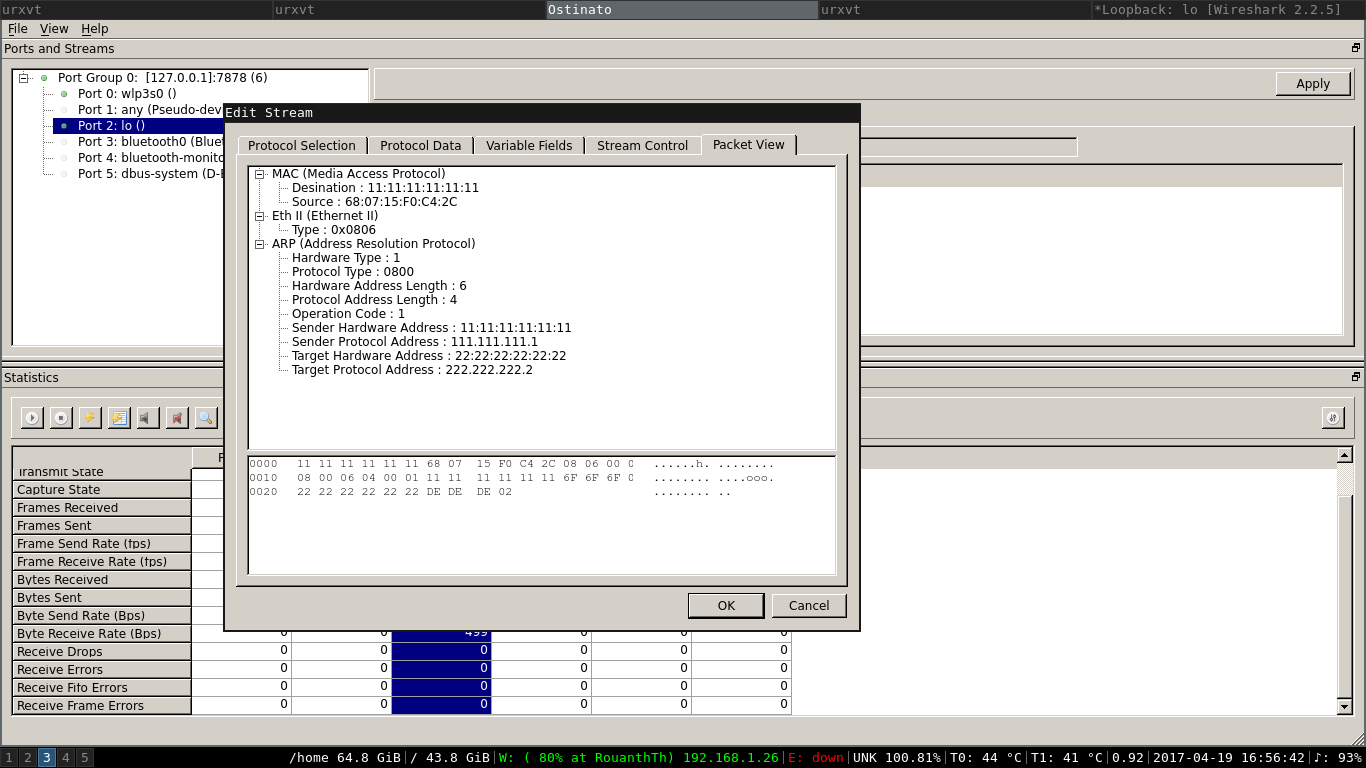
\includegraphics[scale=0.5]{ARPStream_without_frag.png}
		\caption{Конфигурация пакета ARP в Ostinato}
		\center
	\end{figure}

	\begin{figure}[h!]
		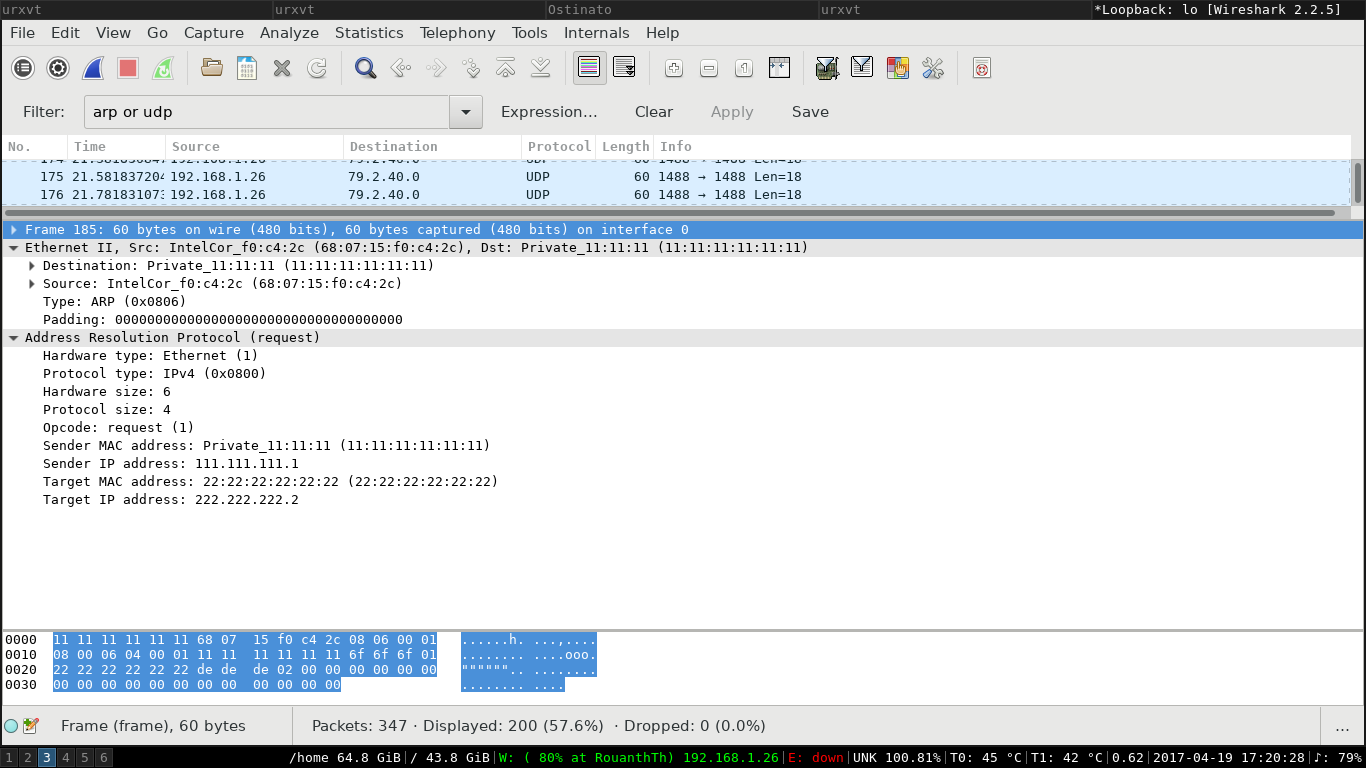
\includegraphics[scale=0.4]{./CapturedARP.png}
		\caption{ARP в Wireshark}
		\center
	\end{figure}

	Фрагментация пакетов не поддерживается в протоколе ARP.

\subsubsection*{UDP}
	UDP (User Datagram Protocol) -- протокол транспортного уровня, использующийся для обмена датаграммами
без установления соединения.

	\begin{figure}[h!]
		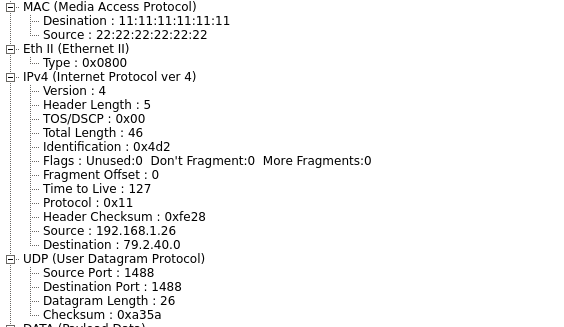
\includegraphics[scale=0.5]{UDPStream_without_frag.png}
		\caption{Конфигурация пакета UDP в Ostinato}
		\center
	\end{figure}

	\begin{figure}[h!]
		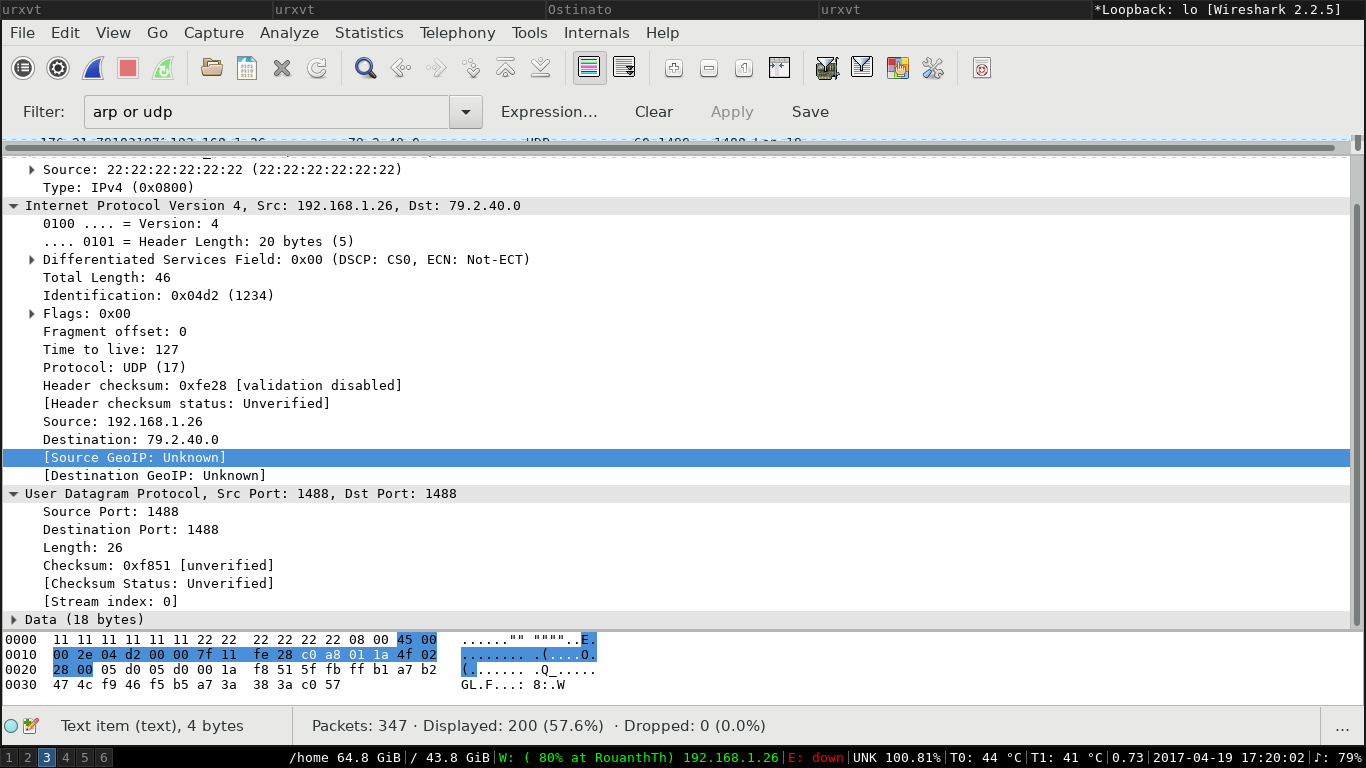
\includegraphics[scale=0.4]{./CapturedUDP.png}
		\caption{UDP в Wireshark}
		\center
	\end{figure}

	\begin{figure}[h!]
		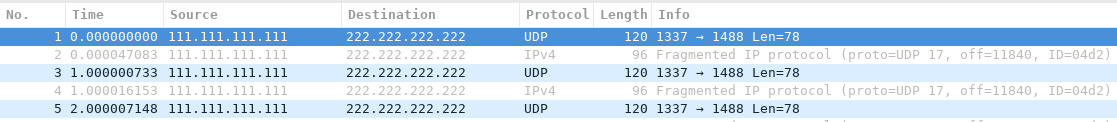
\includegraphics[scale=0.4]{./UDPFrag.png}
		\caption{Фрагемнатция для UDP}
		\center
	\end{figure}

\subsubsection*{Конфигурации трафика}
	Рассмотрим трафик с двумя режимами. \\

	\begin{figure}[h!]
		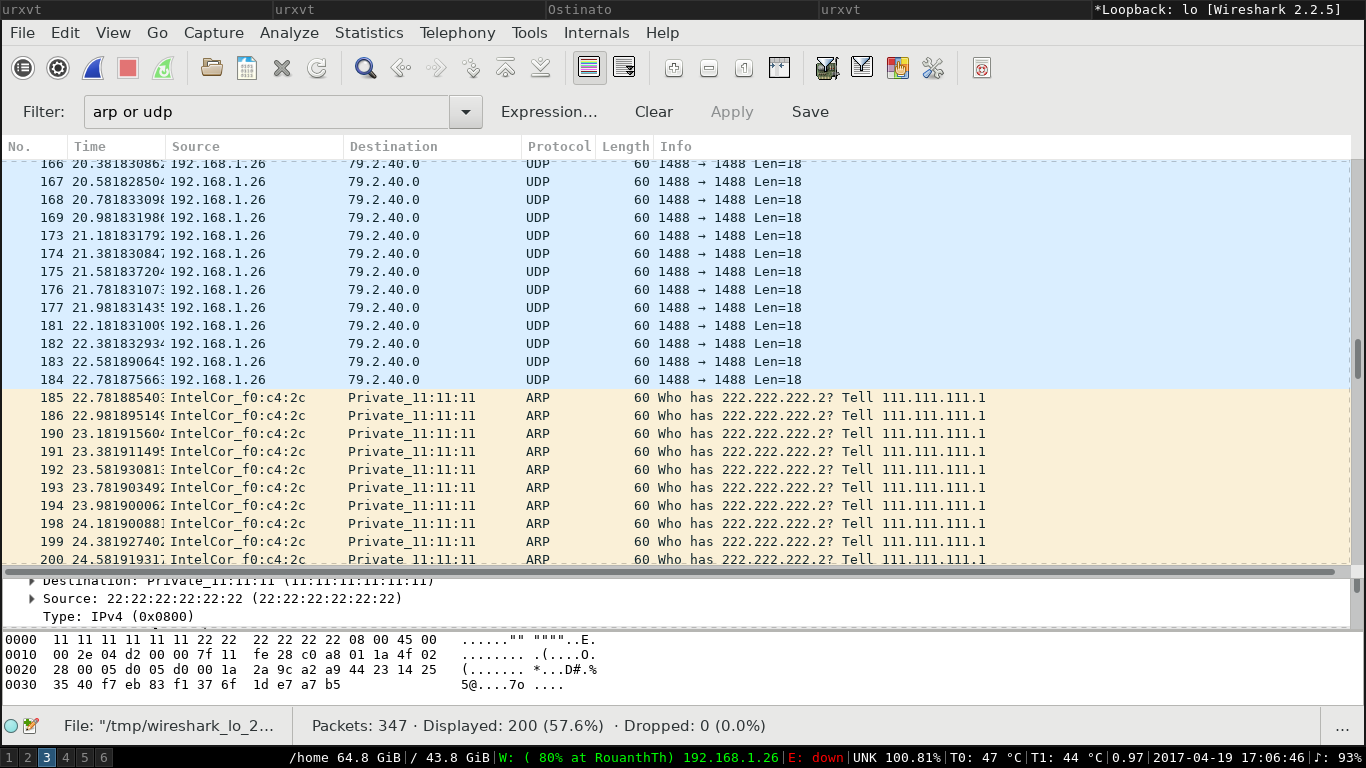
\includegraphics[scale=0.4]{Seq.png}
		\caption{Sequential Streams}
		\center
	\end{figure}

	\begin{figure}[h!]
		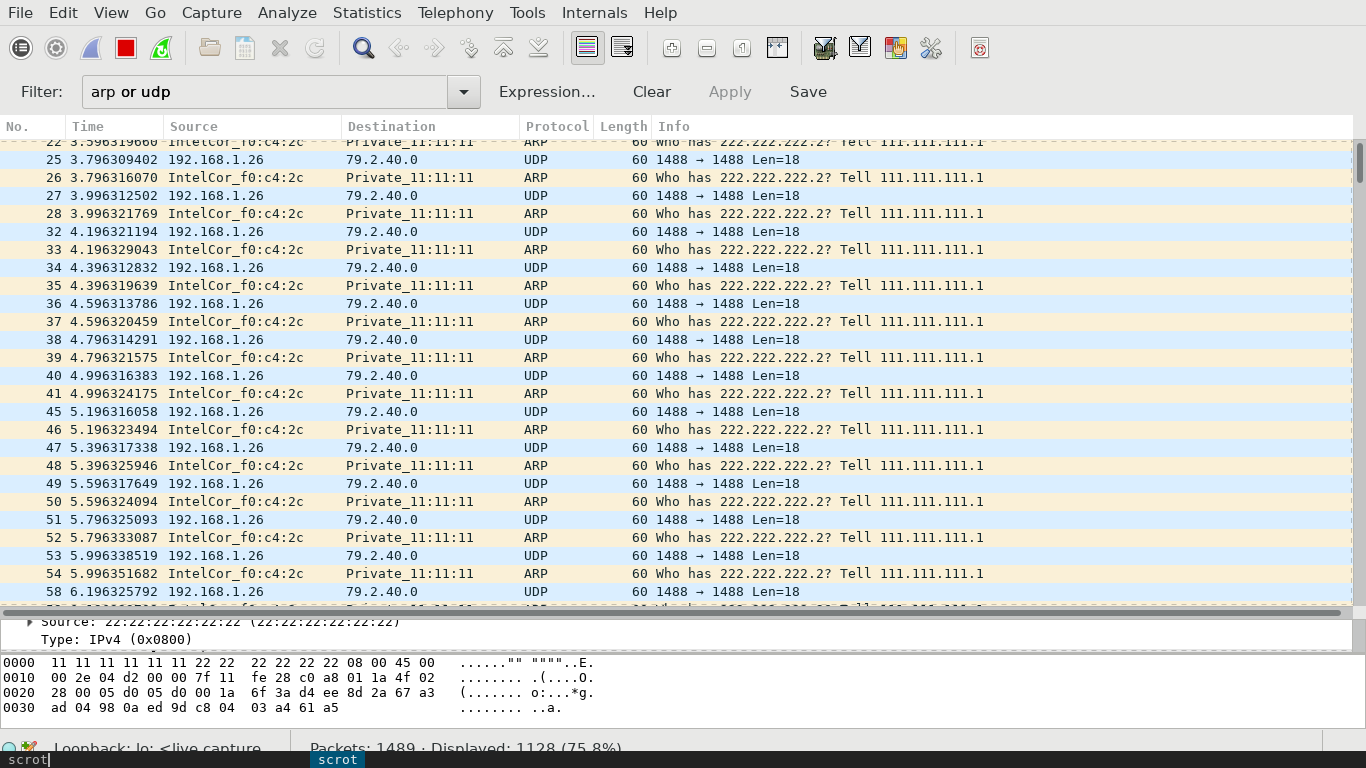
\includegraphics[scale=0.4]{Interleave.png}
		\caption{Interleaved Streams}
		\center
	\end{figure}

	Пойманный Wireshark трафик говорит нам о том, что Ostinato действует в соответствии с
	документацией. \\

\subsection*{Часть Б}

\subsubsection*{IPv4}
	
	Генерация пакетов IPv4. \\

	\begin{figure}[h!]
		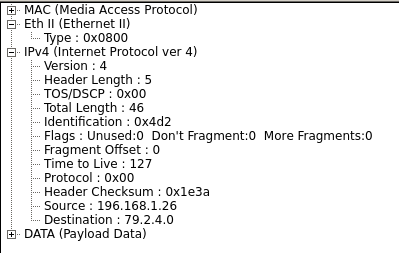
\includegraphics[scale=0.5]{IPStream_without_frag.png}
		\caption{Конфигурация пакета IP в Ostinato}
		\center
	\end{figure}

	\begin{figure}[h!]
		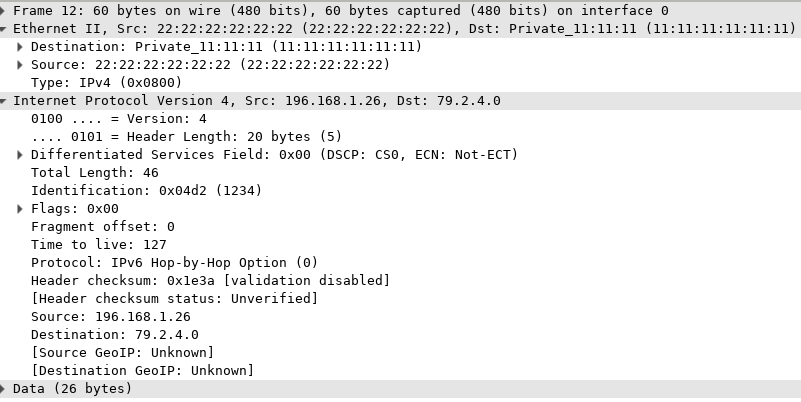
\includegraphics[scale=0.4]{CapturedIP.png}
		\caption{IP в Wireshark}
		\center
	\end{figure}
	\begin{figure}[h!]
		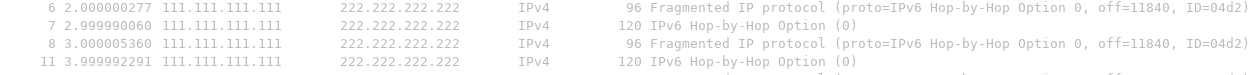
\includegraphics[scale=0.4]{./IPv4Frag.png}
		\caption{Фрагемнатция для IPv4}
		\center
	\end{figure}

\subsubsection*{ICMP}

	Генерация пакетов ICMPv4.  \\
	\begin{figure}[h!]
		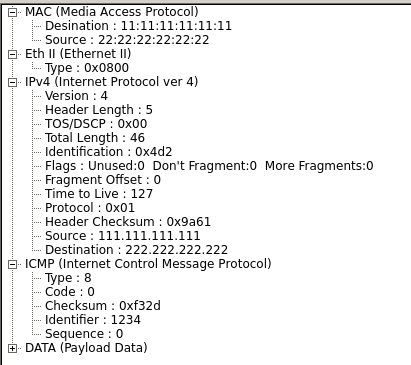
\includegraphics[scale=0.5]{ICMPStream_without_frag.png}
		\caption{Конфигурация пакета ICMP в Ostinato}
		\center
	\end{figure}

	\begin{figure}[h!]
		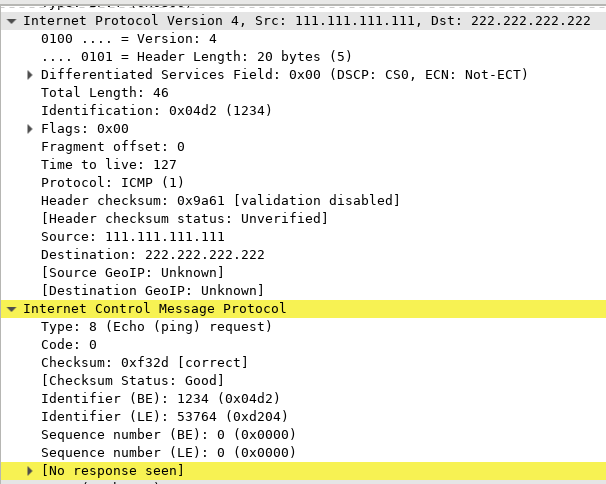
\includegraphics[scale=0.4]{CapturedICMP.png}
		\caption{ICMP в Wireshark}
		\center
	\end{figure}
	\begin{figure}[h!]
		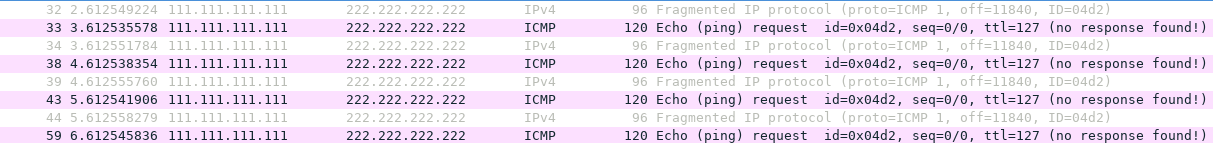
\includegraphics[scale=0.4]{./ICMPFrag.png}
		\caption{Фрагемнатция для ICMP}
		\center
	\end{figure}
\subsubsection*{Конфигурации трафика}
	Рассмотрим трафик с двумя режимами.
	\begin{figure}[h!]
		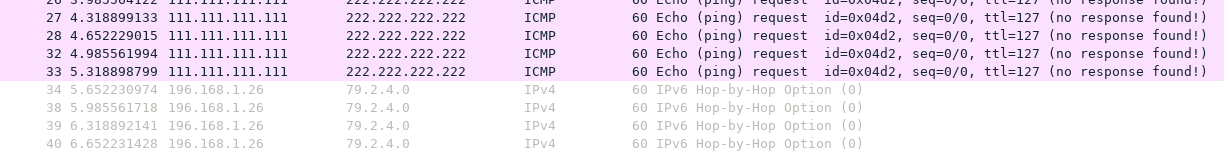
\includegraphics[scale=0.4]{SeqB.png}
		\caption{Sequential Streams}
		\center
	\end{figure}

	\begin{figure}[h!]
		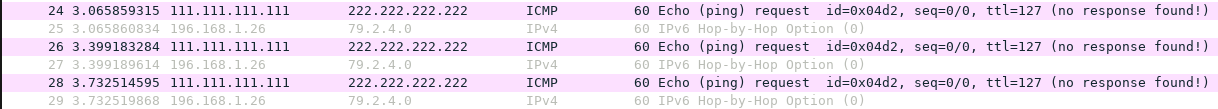
\includegraphics[scale=0.4]{InterleavedB.png}
		\caption{Interleaved Streams}
		\center
	\end{figure}

	Пойманный Wireshark трафик говорит нам о том, что Ostinato действует в соответствии с
	документацией.

\section*{Вывод}

При выполнении лабораторной работы производилось исследование структуры сетевых пакетов с помощью Wireshark и Ostinato.
В результате выполнения работы были сделаны следующие выводы и подмечены следующие детали. 
\begin{enumerate}
	\item \texttt{traceroute} на каждый TTL отправляет три пакета в силу не совсем очевидных причин;
		  скорее всего, для точности результатов и повышения вероятности ответа.
	\item Есть несколько методов работы traceroute: помимо ICMP-метода существует UDP-подход, при котором
		  при запросе отсылается простой UDP-пакет с TTL=1 и максимальным возможным значением порта (32767);
		  разработчики утверждают, что они надеются[1], что узел не примет target-порт и в ответ отошлёт
		  ICMP Destination Unreachable. Данный метод испольуется при предположении, что ICMP Echo Server
		  может быть не доступен на узле (к примеру, отключён администратором[1]).
	\item Для ответа на ICMP Echo каждый узел согласно RFC-1122 должен реализовать ICMP Echo Server.
	\item ARP не работает с IPv6; его функции выполняет ICMPv6.
\end{enumerate}

\section*{Список литературы}
\begin{enumerate}
	\item <<Comparing ICMP and  UDP Traceroute Methods>>, ftp://ftp.hp.com/pub/hpcp/UDP-ICMP-Traceroutes.pdf
	\item https://tools.ietf.org/html/
\end{enumerate}
\end{document} 
